
The European Centre for Nuclear Research (CERN) is one of the largest organisations performing scientific research in fundamental physics. It aims at providing particle accelerator facilities for numerous experiments conducted in a strong international collaboration. The Organisation is situated in the Franco-Swiss border in the Geneva area. Since 2008, CERN has been in possession of the largest particle accelerator ever built, called Large Hadron Collider (LHC). It was attached to the remainder of the CERN accelerator complex. As illustrated in Fig.~\ref{fig:schematic_representation_lhc}, the  accelerator consists of two 27-km rings in which particles travel in opposite directions and accelerate over multiple turns. 

\begin{figure}[H]
    \centering
    \begin{tikzpicture}
    \node at (0,0) {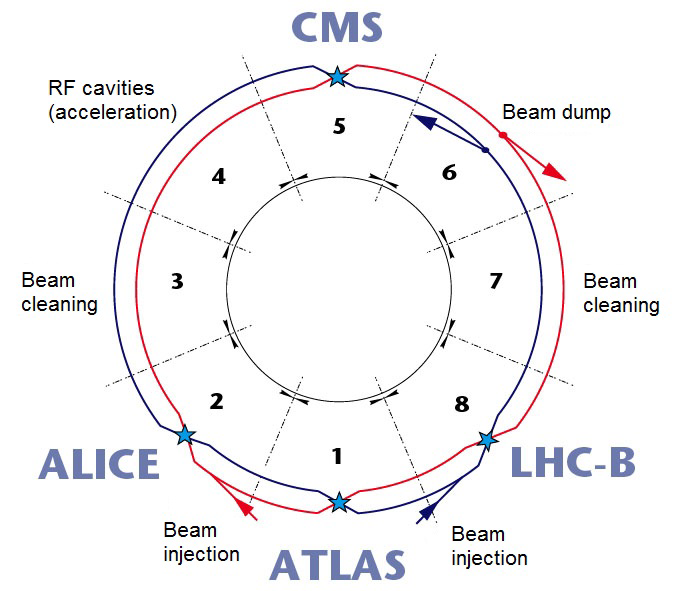
\includegraphics[width=.48\textwidth]{sections/introduction/figures/LHC_accelerator_view.png}};
    \end{tikzpicture}
    \caption{Schematic representation of the LHC~\cite{schematic_representation_lhc}.}
    \label{fig:schematic_representation_lhc}
\end{figure}

The LHC is able to accelerate protons to the energy of $E=7~\text{TeV}$ in each of two rings.  Using two separate loops serves for doubling the collision energy reaching $E=14~\text{TeV}$ at intersection points of the machine. The higher energy is attained, the deeper one can study the particle showers obtained during the impact. They allow for unravelling the fundamentals of particles and interactions between them. There are four collision points in the LHC with different dectectors installed: ATLAS\footnote{A Toroidal LHC ApparatuS}, CMS\footnote{CMS -- Compact Muon Solenoid}, ALICE\footnote{ALICE - A Large Ion Collider Experiment} and LHCb. ATLAS and CMS are two large general-purpose detectors whereas ALICE is specialised in heavy-ion physics and LHCb -- in matter-antimatter asymmetry~\cite[p.~3-21]{evans_marvel_of_technology}.

As presented in Fig.~\ref{fig:schematic_representation_lhc}, the LHC machine is divided into eight sectors. Detectors are installed in four of them. The sectors two and eight serve for inserting the preliminary accelerated beam from other CERN accelerators. In sector four, RF cavities accelerate the beam at every turn before the particles reach the desired energy. The LHC is also equipped with a beam dump system which extracts the beam from the tunnel in case of a machine failure or if the beam quality deteriorates~\cite[p.~1-4]{maciejewski_cosimulation_transient_effects_in_magnets}. 

The LHC is currently being upgraded to the High-Luminosity LHC. The project aims at increasing the frequency of particle collisions which will improve the machine performance. 